% Options for packages loaded elsewhere
\PassOptionsToPackage{unicode}{hyperref}
\PassOptionsToPackage{hyphens}{url}
%
\documentclass[
  ignorenonframetext,
]{beamer}
\usepackage{pgfpages}
\setbeamertemplate{caption}[numbered]
\setbeamertemplate{caption label separator}{: }
\setbeamercolor{caption name}{fg=normal text.fg}
\beamertemplatenavigationsymbolsempty
% Prevent slide breaks in the middle of a paragraph
\widowpenalties 1 10000
\raggedbottom
\setbeamertemplate{part page}{
  \centering
  \begin{beamercolorbox}[sep=16pt,center]{part title}
    \usebeamerfont{part title}\insertpart\par
  \end{beamercolorbox}
}
\setbeamertemplate{section page}{
  \centering
  \begin{beamercolorbox}[sep=12pt,center]{part title}
    \usebeamerfont{section title}\insertsection\par
  \end{beamercolorbox}
}
\setbeamertemplate{subsection page}{
  \centering
  \begin{beamercolorbox}[sep=8pt,center]{part title}
    \usebeamerfont{subsection title}\insertsubsection\par
  \end{beamercolorbox}
}
\AtBeginPart{
  \frame{\partpage}
}
\AtBeginSection{
  \ifbibliography
  \else
    \frame{\sectionpage}
  \fi
}
\AtBeginSubsection{
  \frame{\subsectionpage}
}
\usepackage{amsmath,amssymb}
\usepackage{lmodern}
\usepackage{ifxetex,ifluatex}
\ifnum 0\ifxetex 1\fi\ifluatex 1\fi=0 % if pdftex
  \usepackage[T1]{fontenc}
  \usepackage[utf8]{inputenc}
  \usepackage{textcomp} % provide euro and other symbols
\else % if luatex or xetex
  \usepackage{unicode-math}
  \defaultfontfeatures{Scale=MatchLowercase}
  \defaultfontfeatures[\rmfamily]{Ligatures=TeX,Scale=1}
\fi
\usetheme[]{Boadilla}
% Use upquote if available, for straight quotes in verbatim environments
\IfFileExists{upquote.sty}{\usepackage{upquote}}{}
\IfFileExists{microtype.sty}{% use microtype if available
  \usepackage[]{microtype}
  \UseMicrotypeSet[protrusion]{basicmath} % disable protrusion for tt fonts
}{}
\makeatletter
\@ifundefined{KOMAClassName}{% if non-KOMA class
  \IfFileExists{parskip.sty}{%
    \usepackage{parskip}
  }{% else
    \setlength{\parindent}{0pt}
    \setlength{\parskip}{6pt plus 2pt minus 1pt}}
}{% if KOMA class
  \KOMAoptions{parskip=half}}
\makeatother
\usepackage{xcolor}
\IfFileExists{xurl.sty}{\usepackage{xurl}}{} % add URL line breaks if available
\IfFileExists{bookmark.sty}{\usepackage{bookmark}}{\usepackage{hyperref}}
\hypersetup{
  pdftitle={Probability and Statistics 101},
  hidelinks,
  pdfcreator={LaTeX via pandoc}}
\urlstyle{same} % disable monospaced font for URLs
\newif\ifbibliography
\usepackage{color}
\usepackage{fancyvrb}
\newcommand{\VerbBar}{|}
\newcommand{\VERB}{\Verb[commandchars=\\\{\}]}
\DefineVerbatimEnvironment{Highlighting}{Verbatim}{commandchars=\\\{\}}
% Add ',fontsize=\small' for more characters per line
\usepackage{framed}
\definecolor{shadecolor}{RGB}{248,248,248}
\newenvironment{Shaded}{\begin{snugshade}}{\end{snugshade}}
\newcommand{\AlertTok}[1]{\textcolor[rgb]{0.94,0.16,0.16}{#1}}
\newcommand{\AnnotationTok}[1]{\textcolor[rgb]{0.56,0.35,0.01}{\textbf{\textit{#1}}}}
\newcommand{\AttributeTok}[1]{\textcolor[rgb]{0.77,0.63,0.00}{#1}}
\newcommand{\BaseNTok}[1]{\textcolor[rgb]{0.00,0.00,0.81}{#1}}
\newcommand{\BuiltInTok}[1]{#1}
\newcommand{\CharTok}[1]{\textcolor[rgb]{0.31,0.60,0.02}{#1}}
\newcommand{\CommentTok}[1]{\textcolor[rgb]{0.56,0.35,0.01}{\textit{#1}}}
\newcommand{\CommentVarTok}[1]{\textcolor[rgb]{0.56,0.35,0.01}{\textbf{\textit{#1}}}}
\newcommand{\ConstantTok}[1]{\textcolor[rgb]{0.00,0.00,0.00}{#1}}
\newcommand{\ControlFlowTok}[1]{\textcolor[rgb]{0.13,0.29,0.53}{\textbf{#1}}}
\newcommand{\DataTypeTok}[1]{\textcolor[rgb]{0.13,0.29,0.53}{#1}}
\newcommand{\DecValTok}[1]{\textcolor[rgb]{0.00,0.00,0.81}{#1}}
\newcommand{\DocumentationTok}[1]{\textcolor[rgb]{0.56,0.35,0.01}{\textbf{\textit{#1}}}}
\newcommand{\ErrorTok}[1]{\textcolor[rgb]{0.64,0.00,0.00}{\textbf{#1}}}
\newcommand{\ExtensionTok}[1]{#1}
\newcommand{\FloatTok}[1]{\textcolor[rgb]{0.00,0.00,0.81}{#1}}
\newcommand{\FunctionTok}[1]{\textcolor[rgb]{0.00,0.00,0.00}{#1}}
\newcommand{\ImportTok}[1]{#1}
\newcommand{\InformationTok}[1]{\textcolor[rgb]{0.56,0.35,0.01}{\textbf{\textit{#1}}}}
\newcommand{\KeywordTok}[1]{\textcolor[rgb]{0.13,0.29,0.53}{\textbf{#1}}}
\newcommand{\NormalTok}[1]{#1}
\newcommand{\OperatorTok}[1]{\textcolor[rgb]{0.81,0.36,0.00}{\textbf{#1}}}
\newcommand{\OtherTok}[1]{\textcolor[rgb]{0.56,0.35,0.01}{#1}}
\newcommand{\PreprocessorTok}[1]{\textcolor[rgb]{0.56,0.35,0.01}{\textit{#1}}}
\newcommand{\RegionMarkerTok}[1]{#1}
\newcommand{\SpecialCharTok}[1]{\textcolor[rgb]{0.00,0.00,0.00}{#1}}
\newcommand{\SpecialStringTok}[1]{\textcolor[rgb]{0.31,0.60,0.02}{#1}}
\newcommand{\StringTok}[1]{\textcolor[rgb]{0.31,0.60,0.02}{#1}}
\newcommand{\VariableTok}[1]{\textcolor[rgb]{0.00,0.00,0.00}{#1}}
\newcommand{\VerbatimStringTok}[1]{\textcolor[rgb]{0.31,0.60,0.02}{#1}}
\newcommand{\WarningTok}[1]{\textcolor[rgb]{0.56,0.35,0.01}{\textbf{\textit{#1}}}}
\usepackage{longtable,booktabs,array}
\usepackage{calc} % for calculating minipage widths
\usepackage{caption}
% Make caption package work with longtable
\makeatletter
\def\fnum@table{\tablename~\thetable}
\makeatother
\setlength{\emergencystretch}{3em} % prevent overfull lines
\providecommand{\tightlist}{%
  \setlength{\itemsep}{0pt}\setlength{\parskip}{0pt}}
\setcounter{secnumdepth}{-\maxdimen} % remove section numbering
\AtBeginSection[]{\begin{frame}\tableofcontents[currentsection]\end{frame}}
\AtBeginSubsection[]{\begin{frame}\tableofcontents[currentsubsection]\end{frame}}
\ifluatex
  \usepackage{selnolig}  % disable illegal ligatures
\fi

\title{Probability and Statistics 101}
\subtitle{Can we ever beat the Casino?}
\author{}
\date{\vspace{-2.5em}}

\begin{document}
\frame{\titlepage}

\hypertarget{objectives}{%
\section{Objectives}\label{objectives}}

\begin{frame}[fragile]
\frametitle{Objectives}

\begin{itemize}
\tightlist
\item
  \textbf{Basic elements of Probability}
\end{itemize}

\begin{quote}
The world is full of randomness. It is hard to predict what will exactly
happen next. However, we can describe the randomness using probability.
We will use a simple game to encapsulate the basic elements of
probability: a sample space, events and probability.
\end{quote}

\begin{itemize}
\tightlist
\item
  \textbf{Basic concepts of Statistics}
\end{itemize}

\begin{quote}
We learn and infer the world using what we have observed.
\end{quote}

\begin{itemize}
\tightlist
\item
  Gambling and probability
\end{itemize}

\begin{quote}
\texttt{Gambling\ shows\ that\ there\ has\ been\ an\ interest\ in\ quantifying\ the\ ideas\ of\ probability\ for\ millennia.}
\end{quote}
\end{frame}

\begin{frame}
\frametitle{Table of Content}

\begin{itemize}
\tightlist
\item
  Probability

  \begin{itemize}
  \tightlist
  \item
    Roulette Game
  \item
    Random variable
  \item
    Expected value and Variance
  \item
    The Law of Large Numbers
  \item
    The Central Limit Theorem
  \item
    Bell Curve, Normal Dist. and Standard Normal
  \item
    Covariance
  \end{itemize}
\item
  Statistics

  \begin{itemize}
  \tightlist
  \item
    Are we being cheated?
  \item
    Confidence intervals
  \item
    Hypotheses tests
  \end{itemize}
\end{itemize}
\end{frame}

\hypertarget{case-study-can-we-ever-beat-the-casino}{%
\section{Case study: Can we ever beat the
casino?}\label{case-study-can-we-ever-beat-the-casino}}

\begin{frame}
\frametitle{Roulette Game}

\begin{columns}
 \column{0.5\linewidth}
   \centering
   \includegraphics[width=\linewidth]{roulette}
  \column{0.5\linewidth}
   \centering
   \begin{itemize}
   \item A wheel 
   \begin{itemize}
      \item 0, 00, 1, ..., 36
      \item 18 numbers: red
      \item 18 numbers: black
      \item 0, 00: green
   \end{itemize}
   \item A ball
   \end{itemize}
 \end{columns}

Spin the wheel in one direction and spin the ball in the opposite
direction. Observe where the ball lands.
\end{frame}

\begin{frame}
\frametitle{Claim 1: A losing game}

There are different ways to bet.

\begin{itemize}
\tightlist
\item
  Bet on one single number
\item
  Bet on red or black
\end{itemize}

\vspace{.2in}

\begin{block}{Claim 1}
One will be for sure losing all the money in hands if playing the Roulette game MANY times.
\end{block}
\end{frame}

\begin{frame}
\frametitle{Claim 2: An unfair game}

I once went to a casino and played Red-Black games

\begin{itemize}
\tightlist
\item
  100 times
\item
  Each time bet \$1.00
\item
  I lost \$28 at the end (Same as lost \$.28 on average)
\end{itemize}

\vspace{.2in}

\begin{block}{Claim 2}
The roulette table is not a fair one!
\end{block}

How to prove the claim?

We need the concept of \textbf{probability} and \textbf{statistics}.
\end{frame}

\hypertarget{probability}{%
\section{Probability}\label{probability}}

\hypertarget{probablity-and-random-variable}{%
\subsection{Probablity and Random
Variable}\label{probablity-and-random-variable}}

\begin{frame}
\frametitle{Probablity}

\begin{itemize}
\item
  In a roulette game, you can not predict where the ball is going to
  land. (Randomness)
\item
  But \ldots{} We know the probability of events

  \begin{itemize}
  \tightlist
  \item
    Probability of seeing a 20 is \(\frac{1}{38}\)
  \item
    Probability of seeing a red is \(\frac{18}{38} = 0.47 < 1/2\)
  \end{itemize}
\item
  What does Prob (seeing a 20) = \(\frac{1}{38}\) mean?
\end{itemize}
\end{frame}

\begin{frame}
\frametitle{Probability}
\framesubtitle{What does Prob (seeing a 20) = $\frac{1}{38}$ mean?}

One way: if one plays 1000 times, 20 will roughly appear
\(1000 \times \frac{1}{38} =26\) times

\emph{Probability of a random event: a long term frequency.}

Key elements:

\begin{itemize}
\tightlist
\item
  a sample space
\item
  events
\item
  probability
\end{itemize}
\end{frame}

\begin{frame}
\frametitle{Random Variables (R.V.)}

\begin{itemize}
\item
  A single number game (straight bet): Odds paid 35 to 1 (Put one dollar
  on a number (say 10) and you will win 35 (and get back your original
  \$1) if 10 appears; or you will lose \$1)
\item
  Let \(X\) be the money won for one dollar bet, it is called a random
  variable.
\item
  What are the possible values and corresponding prob?
  \[X=35 \quad \mbox{or} \quad X=-1\]
\item
  Random variables are functions of the sample space.
\end{itemize}
\end{frame}

\begin{frame}
\frametitle{Distributions}

\begin{itemize}
\item
  The possible values together with their probabilities is called the
  distribution

  \begin{itemize}
  \tightlist
  \item
    If we win: \(X = 35\) with prob \(\frac{1}{38}\)
  \item
    If we lose: \(X = -1\) with prob
    \(1 - \frac{1}{38} = \frac{37}{38}\)
  \end{itemize}
\item
  On average how much do you expect that we will win?
\end{itemize}
\end{frame}

\hypertarget{expectation}{%
\subsection{Expectation}\label{expectation}}

\begin{frame}
\frametitle{Expected Value}

\begin{itemize}
\tightlist
\item
  On average how much do you expect that we will win?
\end{itemize}

\[\begin{split}
E(X)& = 35\times \frac{1}{38} +(-1)\times\frac{37}{38} \\
& =\frac{35}{38}-\frac{37}{38} =- \frac{2}{38} =-.0526  
\end{split}\]

\begin{itemize}
\item
  Jargon: \(-.0526\) is called the \textbf{expected} value of \(X\). It
  is the weighted average of \(X\) and is denoted by \(E(X)\).
\item
  Question: What does -.0526 tell us?
\end{itemize}
\end{frame}

\begin{frame}
\frametitle{Another game: Red-Black | Odds paid 1 to 1}

\begin{itemize}
\item
  Put one dollar on one color, say red. If any of the red numbers
  appears you win \$1, otherwise you lose \$1
\item
  Let \(Y\) be the money won for one dollar bet.

  \begin{itemize}
  \tightlist
  \item
    If we win: \(Y = 1\) with prob \(\frac{18}{38}\)
  \item
    If we lose: \(Y = -1\) with prob
    \(1 - \frac{18}{38} = \frac{20}{38}\)
  \end{itemize}
\item
  The expected winning is now \[\begin{split}
   E(X)& = 1\times \frac{18}{38} +(-1)\times\frac{20}{38} =- \frac{2}{38} =-.0526   
   \end{split}\]
\item
  \emph{This is same as the expected winning of one number game!!!!!}
\end{itemize}
\end{frame}

\begin{frame}
\frametitle{Interpretation of Expected Value}

\begin{itemize}
\item
  When we play Red-Black games on one dollar bet, we expect to win
  -0.0526, that is, on average we are going to lose 5.26 cents.
\item
  Let us see what does -0.0526 mean.

  I was in Las Vegas not too long ago and I played Red-Black game 200
  times. I only bet one dollar each time.
\end{itemize}
\end{frame}

\begin{frame}
\frametitle{Interpretation of Expected Value}

\begin{itemize}
\tightlist
\item
  Here is the summary of the 200 Red-Black games:
\end{itemize}

\begin{longtable}[]{@{}
  >{\raggedright\arraybackslash}p{(\columnwidth - 4\tabcolsep) * \real{0.33}}
  >{\raggedright\arraybackslash}p{(\columnwidth - 4\tabcolsep) * \real{0.33}}
  >{\raggedright\arraybackslash}p{(\columnwidth - 4\tabcolsep) * \real{0.33}}@{}}
\toprule
\(\;\) & Actual & Expected \\
\midrule
\endhead
Lost & 105 times & \(200 \times \frac{20}{38} = 105.3\) \\
Won & 95 times & \(200 \times \frac{18}{38} = 94.7\) \\
Average Winning &
\(\bar{Y}_{200} = \frac{Y_1 + \ldots+ Y_{200}}{200} = (-105+95)/200=-0.050\)
& -0.0526 \\
\bottomrule
\end{longtable}
\end{frame}

\begin{frame}
\Large
\begin{center}
Are you surprised to see this?
\end{center}
\end{frame}

\hypertarget{law-of-large-numbers}{%
\subsection{Law of Large Numbers}\label{law-of-large-numbers}}

\begin{frame}[fragile]{Law of Large Numbers}
\begin{longtable}[]{@{}
  >{\raggedright\arraybackslash}p{(\columnwidth - 0\tabcolsep) * \real{0.06}}@{}}
\toprule
\endhead
\textbackslash frametitle\{Behavior of Long Term Frequency\$\} \\
\small \\
\texttt{r\ n\ \textless{}-\ 200\ win\_prob\ \textless{}-\ 18/38\ \#\ winning\ event\ set.seed(2021)\ win\_vec\ \textless{}-\ rbinom(n,1,win\_prob)\ \#\ rbinom(1,1,\ win\_prob)\ \ \ \#one\ game\ at\ a\ time\ \#\ cumulative\ mean\ =\ cumulative\ sum\ /\ cumulative\ number\ of\ games\ cum\_mean\ \textless{}-\ cumsum(win\_vec)/(1:n)\ \#\ data.frame\ cum\_mean\_df\ \textless{}-\ data.frame(num\_of\_games\ =\ 1:n,\ cum\_mean\ =\ cum\_mean)\ head(cum\_mean\_df)} \\
\texttt{\#\#\ \ \ num\_of\_games\ \ cum\_mean\ \#\#\ 1\ \ \ \ \ \ \ \ \ \ \ \ 1\ 0.0000000\ \#\#\ 2\ \ \ \ \ \ \ \ \ \ \ \ 2\ 0.5000000\ \#\#\ 3\ \ \ \ \ \ \ \ \ \ \ \ 3\ 0.6666667\ \#\#\ 4\ \ \ \ \ \ \ \ \ \ \ \ 4\ 0.5000000\ \#\#\ 5\ \ \ \ \ \ \ \ \ \ \ \ 5\ 0.6000000\ \#\#\ 6\ \ \ \ \ \ \ \ \ \ \ \ 6\ 0.6666667} \\
\bottomrule
\end{longtable}

\frametitle{Behavior of Long Term Frequency}

\scriptsize

\begin{Shaded}
\begin{Highlighting}[]
\FunctionTok{ggplot}\NormalTok{(cum\_mean\_df, }
     \FunctionTok{aes}\NormalTok{(}\AttributeTok{x =}\NormalTok{ num\_of\_games, }\AttributeTok{y =}\NormalTok{ cum\_mean)) }\SpecialCharTok{+}
\FunctionTok{geom\_line}\NormalTok{() }\SpecialCharTok{+} \FunctionTok{geom\_point}\NormalTok{() }\SpecialCharTok{+}
\FunctionTok{geom\_hline}\NormalTok{(}\AttributeTok{yintercept =}\NormalTok{ win\_prob, }\AttributeTok{col =} \StringTok{"red"}\NormalTok{) }\SpecialCharTok{+}
\CommentTok{\# xlab("Number of games") + }
\FunctionTok{ylab}\NormalTok{(}\StringTok{"Average winning percentage"}\NormalTok{) }\SpecialCharTok{+}
\FunctionTok{scale\_y\_continuous}\NormalTok{(}\AttributeTok{labels =}\NormalTok{ percent) }\SpecialCharTok{+}
\FunctionTok{theme\_bw}\NormalTok{()}
\end{Highlighting}
\end{Shaded}

\begin{center}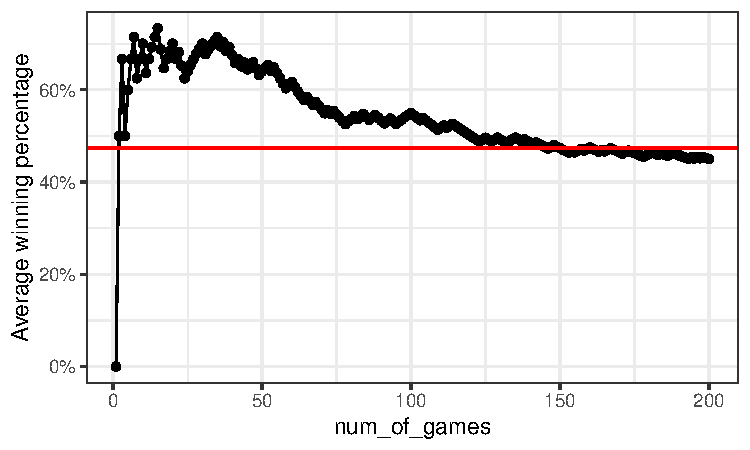
\includegraphics[width=0.7\linewidth]{Probability_Statistics_101_v2_files/figure-beamer/unnamed-chunk-2-1} \end{center}
\end{frame}

\begin{frame}[fragile]
\frametitle{Behavior of Sample Mean $\bar{Y}_{n}$}
\scriptsize

\begin{Shaded}
\begin{Highlighting}[]
\CommentTok{\# expected gain}
\NormalTok{expected\_gain }\OtherTok{\textless{}{-}}\NormalTok{ win\_prob }\SpecialCharTok{{-}}\NormalTok{ (}\DecValTok{1}\SpecialCharTok{{-}}\NormalTok{win\_prob)}

\CommentTok{\# if win: +1; if lose: {-}1}
\NormalTok{gain\_vec }\OtherTok{\textless{}{-}}\NormalTok{ win\_vec}\SpecialCharTok{*}\DecValTok{2{-}1}

\CommentTok{\# sample() function:}
\CommentTok{\# x: elements to choose; size: repeat how many times; }
\CommentTok{\# replace: sample with replacement; prob: probability to choose each x}
\NormalTok{gain\_vec }\OtherTok{\textless{}{-}} \FunctionTok{sample}\NormalTok{(}\AttributeTok{x =} \FunctionTok{c}\NormalTok{(}\DecValTok{1}\NormalTok{,}\SpecialCharTok{{-}}\DecValTok{1}\NormalTok{), }
                 \AttributeTok{size =}\NormalTok{ n,}
                 \AttributeTok{replace =}\NormalTok{ T, }
                 \AttributeTok{prob =} \FunctionTok{c}\NormalTok{(win\_prob, }\DecValTok{1}\SpecialCharTok{{-}}\NormalTok{ win\_prob))}

\NormalTok{gain\_vec}
\end{Highlighting}
\end{Shaded}

\begin{verbatim}
##   [1] -1 -1  1  1 -1 -1 -1 -1 -1 -1 -1 -1 -1 -1 -1 -1 -1 -1  1  1  1  1 -1  1 -1
##  [26] -1  1  1 -1  1  1 -1  1 -1  1 -1  1  1 -1  1  1  1 -1 -1 -1  1 -1  1  1 -1
##  [51]  1 -1  1 -1  1 -1  1  1  1 -1 -1 -1  1  1  1 -1 -1 -1  1 -1 -1 -1  1  1 -1
##  [76]  1  1 -1 -1 -1 -1  1  1 -1 -1  1 -1 -1  1 -1 -1  1 -1 -1  1 -1 -1  1  1  1
## [101] -1 -1 -1 -1 -1 -1  1  1 -1  1 -1  1 -1 -1  1  1 -1 -1 -1 -1  1  1  1 -1  1
## [126] -1  1  1 -1  1 -1 -1 -1  1  1 -1  1  1  1 -1  1  1 -1 -1 -1  1  1 -1 -1 -1
## [151]  1  1  1 -1  1  1 -1 -1  1  1 -1 -1 -1  1  1  1  1  1  1  1 -1  1  1  1  1
## [176]  1  1 -1  1 -1 -1  1  1 -1  1  1 -1  1  1 -1 -1 -1 -1 -1  1 -1 -1 -1  1 -1
\end{verbatim}
\end{frame}

\begin{frame}[fragile]
\frametitle{Behavior of $\bar{Y}_{n}$ }

\begin{Shaded}
\begin{Highlighting}[]
\CommentTok{\# average gain}
\NormalTok{ave\_gain }\OtherTok{\textless{}{-}} \FunctionTok{cumsum}\NormalTok{(gain\_vec)}\SpecialCharTok{/}\DecValTok{1}\SpecialCharTok{:}\NormalTok{n}

\CommentTok{\# data.frame}
\NormalTok{cum\_gain\_df }\OtherTok{\textless{}{-}} \FunctionTok{data.frame}\NormalTok{(}\AttributeTok{num\_of\_games =} \DecValTok{1}\SpecialCharTok{:}\NormalTok{n,}
                        \AttributeTok{ave\_gain =}\NormalTok{ ave\_gain)}
\end{Highlighting}
\end{Shaded}

\begin{Shaded}
\begin{Highlighting}[]
\CommentTok{\# plot}
\FunctionTok{ggplot}\NormalTok{(cum\_gain\_df, }
     \FunctionTok{aes}\NormalTok{(}\AttributeTok{x =}\NormalTok{ num\_of\_games, }\AttributeTok{y =}\NormalTok{ ave\_gain)) }\SpecialCharTok{+}
\FunctionTok{geom\_line}\NormalTok{() }\SpecialCharTok{+} \FunctionTok{geom\_point}\NormalTok{() }\SpecialCharTok{+}
\FunctionTok{geom\_hline}\NormalTok{(}\AttributeTok{yintercept =}\NormalTok{ expected\_gain, }\AttributeTok{col =} \StringTok{"darkgreen"}\NormalTok{) }\SpecialCharTok{+}
\FunctionTok{xlab}\NormalTok{(}\StringTok{"Number of games"}\NormalTok{) }\SpecialCharTok{+} 
\FunctionTok{ylab}\NormalTok{(}\StringTok{"Average winning"}\NormalTok{) }\SpecialCharTok{+}
\FunctionTok{theme\_bw}\NormalTok{()}
\end{Highlighting}
\end{Shaded}
\end{frame}

\begin{frame}
\frametitle{Behavior of $\bar{Y}_{n}$ }

\begin{center}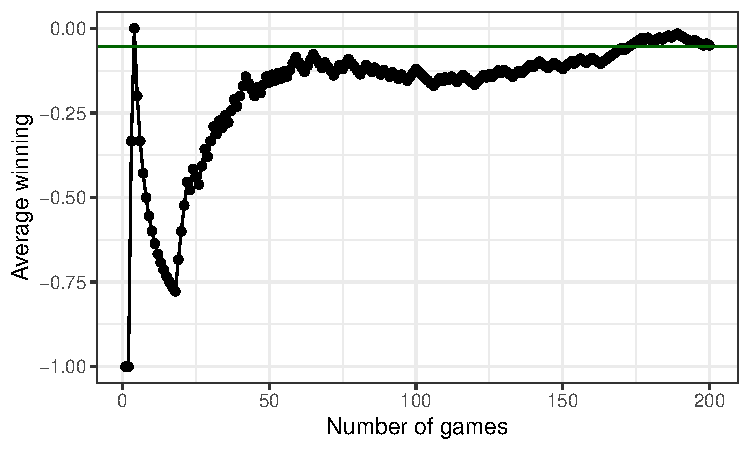
\includegraphics[width=0.7\linewidth]{Probability_Statistics_101_v2_files/figure-beamer/unnamed-chunk-6-1} \end{center}
\end{frame}

\begin{frame}
\frametitle{Law of Large Numbers}

\begin{itemize}
\item
  The expected winning for Red-Black game is -0.0526
\item
  Long term Average \(\approx\) expected value
\end{itemize}

\[\bar{Y}_{n} \rightarrow \mu \mbox{ or } E(Y) \mbox{ (Expected value)}\]
\end{frame}

\begin{frame}
\frametitle{Which game is better?}

\begin{itemize}
\item
  The expected winning for Red-Black game is -0.0526
\item
  Recall that the expected winning for Single number bet is also -0.0526
\item
  Both games have the same expected values.
\end{itemize}

\begin{center}
Which game should we play to make money?
\end{center}
\end{frame}

\hypertarget{variance}{%
\subsection{Variance}\label{variance}}

\begin{frame}
\frametitle{Risk measurement: Variance}

\Large
\begin{center}
HOW?
Little long stories!
\end{center}
\end{frame}

\begin{frame}
\frametitle{Variability: Variance}

\begin{itemize}
\item
  X=winning on a single number bet: It can be 35 or -1 with prob 1/38 or
  37/38. The expected winning is -0.0526
\item
  Variance: the expected squared difference of the winning from the
  expected winning =\(E(X -\mu)^2=\sigma^2=VAR(X)\):
  \[\scriptstyle {\sigma_X^2 = (35 -(- 0.0526))^2 \times \frac{1}{38} +  (- 1 -(- 0.0526))^2  \times \frac{37}{38} = 33.208} \]
\item
  Standard Deviation:
  \[\scriptstyle \sqrt{\sigma_X^2}  = \sqrt{33.208} = 5.76 \]
\end{itemize}

Notice: Expected values and Variances are theoretical quantities. They
are different from sample means and sample variances.
\end{frame}

\begin{frame}
\frametitle{Standard Deviation for Y, the winning for Red-Black game?}

\begin{itemize}
\item
  Y takes value 1 and -1 with prob. 18/38 and 20/38
\item
  \[\scriptstyle Var(Y)=(1 - (- 0.0526))^2  \times \frac{18}{38} + (- 1 -(- 0.0526))^2 \times \frac{20}{38} = 0.997\]
\item
  \[\scriptstyle \sigma_Y = \sqrt{0.997} =  0.998\]
\item
  The variability of winning from a single number game (SD=5.76) is much
  larger than that of Red-Black (SD=0.998)
\item
  How do Variances help us to determine which game to play?
\end{itemize}
\end{frame}

\hypertarget{central-limit-theorem-clt}{%
\subsection{Central Limit Theorem
(CLT)}\label{central-limit-theorem-clt}}

\begin{frame}
\frametitle{Behavior of the average winning}

(Sample of size 10, 100, 10000 vs.~the population)

We all play Red-Black game, bet one dollar each time

\begin{itemize}
\tightlist
\item
  \(\bar{Y}_{10}\), each person play 10 times 48 of us
\item
  \(\bar{Y}_{100}\), each person play 100 times 48 of us
\item
  \(\bar{Y}_{10,000}\), each person play 10,000 times 48 of us
\end{itemize}
\end{frame}

\begin{frame}[fragile]
\frametitle{Behavior of the average winning}
\tiny

\begin{Shaded}
\begin{Highlighting}[]
\NormalTok{n\_times }\OtherTok{\textless{}{-}} \DecValTok{48}
\NormalTok{win\_prob }\OtherTok{\textless{}{-}} \DecValTok{18}\SpecialCharTok{/}\DecValTok{38}

\CommentTok{\# create a data frame}
\DocumentationTok{\#\# 10 times}
\FunctionTok{set.seed}\NormalTok{(}\DecValTok{1}\NormalTok{)}
\NormalTok{avg\_winning\_df\_10 }\OtherTok{\textless{}{-}}
  \FunctionTok{data.frame}\NormalTok{(}\AttributeTok{id =} \DecValTok{1}\SpecialCharTok{:}\NormalTok{n\_times,}
             \AttributeTok{n =} \DecValTok{10}\NormalTok{, }
             \AttributeTok{num\_win =} \FunctionTok{rbinom}\NormalTok{(n\_times, }\DecValTok{10}\NormalTok{, win\_prob))}
\DocumentationTok{\#\# 100 times}
\NormalTok{avg\_winning\_df\_100 }\OtherTok{\textless{}{-}} 
  \FunctionTok{data.frame}\NormalTok{(}\AttributeTok{id =} \DecValTok{1}\SpecialCharTok{:}\NormalTok{n\_times,}
             \AttributeTok{n =} \DecValTok{100}\NormalTok{, }
             \AttributeTok{num\_win =} \FunctionTok{rbinom}\NormalTok{(n\_times, }\DecValTok{100}\NormalTok{, win\_prob))}

\CommentTok{\# 10000 times}
\NormalTok{avg\_winning\_df\_10000 }\OtherTok{\textless{}{-}} 
  \FunctionTok{data.frame}\NormalTok{(}\AttributeTok{id =} \DecValTok{1}\SpecialCharTok{:}\NormalTok{n\_times, }
             \AttributeTok{n =} \DecValTok{10000}\NormalTok{, }
             \AttributeTok{num\_win =} \FunctionTok{rbinom}\NormalTok{(n\_times, }\DecValTok{10000}\NormalTok{, win\_prob))}

\NormalTok{avg\_winning\_df }\OtherTok{\textless{}{-}} \FunctionTok{rbind}\NormalTok{(avg\_winning\_df\_10, avg\_winning\_df\_100, avg\_winning\_df\_10000)}

\NormalTok{avg\_winning\_df }\OtherTok{\textless{}{-}} 
\NormalTok{  avg\_winning\_df }\SpecialCharTok{\%\textgreater{}\%}
  \FunctionTok{mutate}\NormalTok{(}\AttributeTok{avg =}\NormalTok{ (num\_win }\SpecialCharTok{{-}}\NormalTok{ (n}\SpecialCharTok{{-}}\NormalTok{num\_win))}\SpecialCharTok{/}\NormalTok{n )}

\DocumentationTok{\#\# another way}
\CommentTok{\# times \textless{}{-} c(10, 100, 10000)}
\CommentTok{\# ns \textless{}{-} rep(times, each = n\_times)}
\CommentTok{\# avg\_winning\_df \textless{}{-} }
\CommentTok{\#   data.frame(id = rep(1:n\_times, 3),}
\CommentTok{\#              n = ns,}
\CommentTok{\#              num\_win = unlist(lapply(times,}
\CommentTok{\#                                  function(x) rbinom(n\_times, x, win\_prob)))}
\CommentTok{\#              ) \%\textgreater{}\%}
\CommentTok{\#   mutate(avg = (num\_win {-} (n{-}num\_win))/n )}
\end{Highlighting}
\end{Shaded}
\end{frame}

\begin{frame}
\frametitle{Behavior of the average winning}
\tiny

\begin{center}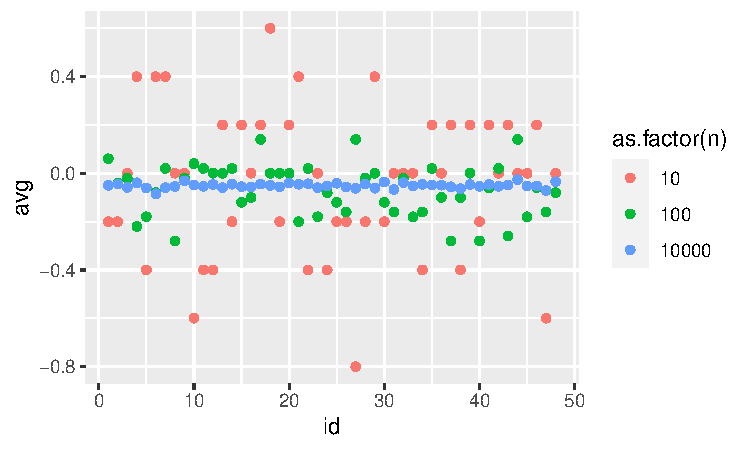
\includegraphics[width=1\linewidth]{Probability_Statistics_101_v2_files/figure-beamer/unnamed-chunk-9-1} \end{center}
\end{frame}

\begin{frame}[fragile]
\frametitle{Behavior of the average winning}

\begin{Shaded}
\begin{Highlighting}[]
\NormalTok{avg\_winning\_df }\SpecialCharTok{\%\textgreater{}\%}
  \FunctionTok{group\_by}\NormalTok{(n) }\SpecialCharTok{\%\textgreater{}\%}
  \FunctionTok{summarize}\NormalTok{(}\AttributeTok{mean =} \FunctionTok{mean}\NormalTok{(avg),}
            \AttributeTok{sd =} \FunctionTok{sd}\NormalTok{(avg),}
            \AttributeTok{total =} \FunctionTok{sum}\NormalTok{(avg}\SpecialCharTok{*}\NormalTok{n))}
\end{Highlighting}
\end{Shaded}

\begin{verbatim}
## # A tibble: 3 x 4
##       n    mean     sd  total
##   <dbl>   <dbl>  <dbl>  <dbl>
## 1    10 -0.0417 0.303     -20
## 2   100 -0.0704 0.109    -338
## 3 10000 -0.0510 0.0104 -24466
\end{verbatim}
\end{frame}

\begin{frame}[fragile]
\frametitle{Behavior of the average winning}
\tiny

\begin{Shaded}
\begin{Highlighting}[]
\FunctionTok{ggplot}\NormalTok{(avg\_winning\_df, }\FunctionTok{aes}\NormalTok{(}\AttributeTok{x =}\NormalTok{ avg, }\AttributeTok{fill =} \FunctionTok{as.factor}\NormalTok{(n))) }\SpecialCharTok{+} 
  \FunctionTok{geom\_histogram}\NormalTok{() }\SpecialCharTok{+}
  \FunctionTok{facet\_wrap}\NormalTok{(}\SpecialCharTok{\textasciitilde{}}\NormalTok{n, }\AttributeTok{nrow =} \DecValTok{1}\NormalTok{)}
\end{Highlighting}
\end{Shaded}

\begin{verbatim}
## `stat_bin()` using `bins = 30`. Pick better value with `binwidth`.
\end{verbatim}

\begin{center}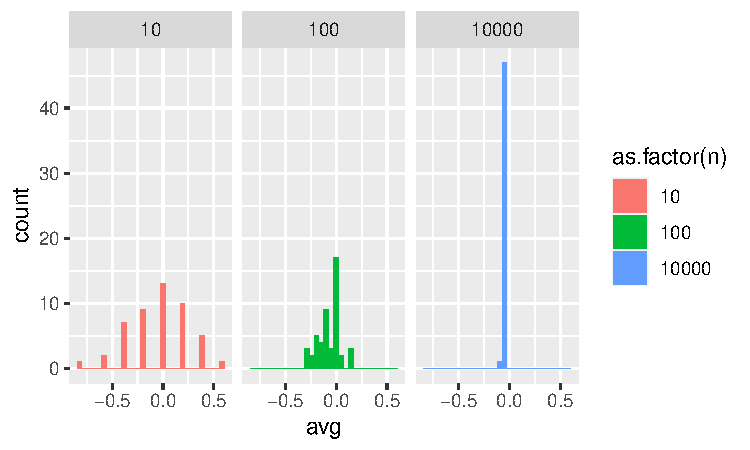
\includegraphics[width=0.9\linewidth]{Probability_Statistics_101_v2_files/figure-beamer/unnamed-chunk-11-1} \end{center}
\end{frame}

\begin{frame}
\frametitle{Central Limit Theorem (CLT)}

\begin{itemize}
\tightlist
\item
  When a large number of games are played

  \begin{itemize}
  \tightlist
  \item
    The average amount each person wins (lost in this case) tends to be
    close to the center = ``expectation'\,' (-0.0526)
  \item
    The distribution is also approximately a bell curve!
  \end{itemize}
\item
  The Central Limit Theorem

  \begin{itemize}
  \tightlist
  \item
    \(\bar{Y}_n\) has a normal distribution
  \item
    \(E[\bar{Y}_n] = \mu /n\)
  \item
    \(Var(\bar{Y}_n) = \sigma^2 /n\)
  \end{itemize}
\item
  Almost for sure each one of us will lose all the money if we keep
  playing!
\end{itemize}
\end{frame}

\begin{frame}
\frametitle{Single number games}

\begin{center}
What about instead we have all played single number games? 
\end{center}
\end{frame}

\begin{frame}[fragile]
\frametitle{Single number game}
\tiny

\begin{Shaded}
\begin{Highlighting}[]
\CommentTok{\# winning probability}
\NormalTok{win\_prob }\OtherTok{=} \DecValTok{1}\SpecialCharTok{/}\DecValTok{38}
\CommentTok{\# number of game}
\NormalTok{n\_times }\OtherTok{\textless{}{-}} \DecValTok{48}
\CommentTok{\# number of trials each game}
\NormalTok{times }\OtherTok{\textless{}{-}} \FunctionTok{c}\NormalTok{(}\DecValTok{10}\NormalTok{, }\DecValTok{100}\NormalTok{, }\DecValTok{10000}\NormalTok{)}
\NormalTok{ns }\OtherTok{\textless{}{-}} \FunctionTok{rep}\NormalTok{(times, }\AttributeTok{each =}\NormalTok{ n\_times)}
\CommentTok{\# number of win}
\NormalTok{num\_win }\OtherTok{\textless{}{-}} \FunctionTok{c}\NormalTok{(}\FunctionTok{sapply}\NormalTok{(times, }
                  \ControlFlowTok{function}\NormalTok{(trial) }\FunctionTok{rbinom}\NormalTok{(n\_times, trial, win\_prob)))}

\NormalTok{avg\_winning\_df }\OtherTok{\textless{}{-}} \FunctionTok{data.frame}\NormalTok{(}\AttributeTok{id =} \FunctionTok{rep}\NormalTok{(}\DecValTok{1}\SpecialCharTok{:}\NormalTok{n\_times, }\DecValTok{3}\NormalTok{),}
                             \AttributeTok{n =}\NormalTok{ ns,}
                             \AttributeTok{num\_win =}\NormalTok{ num\_win)}

\NormalTok{avg\_winning\_df }\OtherTok{\textless{}{-}} 
\NormalTok{  avg\_winning\_df }\SpecialCharTok{\%\textgreater{}\%}
  \FunctionTok{mutate}\NormalTok{(}\AttributeTok{avg =}\NormalTok{ (num\_win}\SpecialCharTok{*}\DecValTok{35} \SpecialCharTok{{-}}\NormalTok{ (n}\SpecialCharTok{{-}}\NormalTok{num\_win))}\SpecialCharTok{/}\NormalTok{n )}
\end{Highlighting}
\end{Shaded}
\end{frame}

\begin{frame}[fragile]
\frametitle{Single number game}

\begin{Shaded}
\begin{Highlighting}[]
\NormalTok{avg\_winning\_df }\SpecialCharTok{\%\textgreater{}\%}
  \FunctionTok{group\_by}\NormalTok{(n) }\SpecialCharTok{\%\textgreater{}\%}
  \FunctionTok{summarize}\NormalTok{(}\AttributeTok{mean =} \FunctionTok{mean}\NormalTok{(avg),}
            \AttributeTok{sd =} \FunctionTok{sd}\NormalTok{(avg),}
            \AttributeTok{total =} \FunctionTok{sum}\NormalTok{(avg}\SpecialCharTok{*}\NormalTok{n))}
\end{Highlighting}
\end{Shaded}

\begin{verbatim}
## # A tibble: 3 x 4
##       n    mean     sd  total
##   <dbl>   <dbl>  <dbl>  <dbl>
## 1    10  0.275  2.29      132
## 2   100 -0.07   0.550    -336
## 3 10000 -0.0674 0.0568 -32340
\end{verbatim}
\end{frame}

\begin{frame}[fragile]
\frametitle{Single number game}
\tiny

\begin{Shaded}
\begin{Highlighting}[]
\FunctionTok{ggplot}\NormalTok{(avg\_winning\_df, }\FunctionTok{aes}\NormalTok{(}\AttributeTok{x =}\NormalTok{ avg, }\AttributeTok{fill =} \FunctionTok{as.factor}\NormalTok{(n))) }\SpecialCharTok{+} 
  \FunctionTok{geom\_histogram}\NormalTok{(}\AttributeTok{bins =} \DecValTok{100}\NormalTok{) }\SpecialCharTok{+}
  \FunctionTok{facet\_wrap}\NormalTok{(}\SpecialCharTok{\textasciitilde{}}\NormalTok{n, }\AttributeTok{nrow =} \DecValTok{1}\NormalTok{)}
\end{Highlighting}
\end{Shaded}

\begin{center}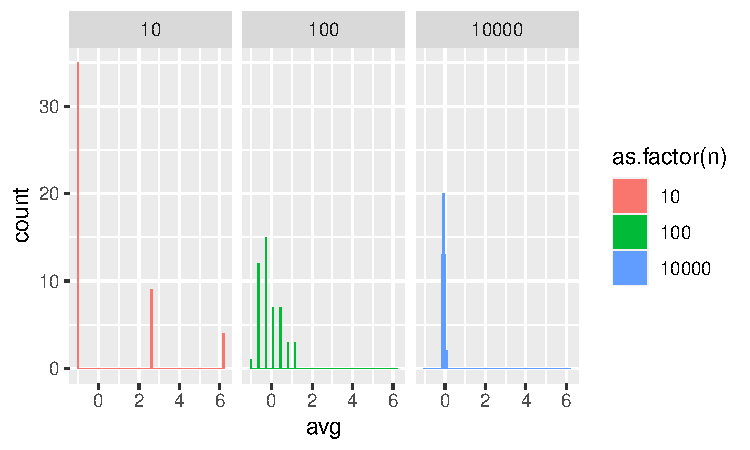
\includegraphics[width=0.9\linewidth]{Probability_Statistics_101_v2_files/figure-beamer/unnamed-chunk-14-1} \end{center}
\end{frame}

\begin{frame}
\frametitle{Summary of two games:  Single number vs Red-Black}

\begin{itemize}
\tightlist
\item
  The expected winning is same: -.0526 on one dollar
\item
  Single number:

  \begin{itemize}
  \tightlist
  \item
    One may have chance to win large amount
  \item
    BUT one may also lose a lot
  \item
    On average you come out the same as Red-Black
  \end{itemize}
\item
  Red-Black:

  \begin{itemize}
  \tightlist
  \item
    Much more conservative
  \item
    If you want to kill time you may choose this game
  \end{itemize}
\end{itemize}

After all: Almost for sure to lose money if one plays many times
\end{frame}

\begin{frame}
\frametitle{Take away:}

\begin{itemize}
\item
  You can not tell for sure what will happen for a random event.
\item
  Probability tells us on average how often the event will occur.
\item
  A random number changes

  \begin{itemize}
  \tightlist
  \item
    The center: expected value
  \item
    The spread: standard deviation
  \end{itemize}
\item
  An average of random sample follows a bell curve

  \begin{itemize}
  \tightlist
  \item
    It tends to the expected value
  \item
    The variability is much smaller when sample size is larger
  \end{itemize}
\end{itemize}
\end{frame}

\hypertarget{bell-curve-and-normal-distribution}{%
\subsection{Bell Curve and Normal
Distribution}\label{bell-curve-and-normal-distribution}}

\begin{frame}
\frametitle{Normal Random Variable}

X = value drawn randomly from a normal population with mean \(\mu\) and
standard deviation \(\sigma\).

\begin{itemize}
\tightlist
\item
  Often abbreviated as \(X \sim N(\mu,\sigma^2)\).
\item
  Density: \[
  f(x) = \frac{1}{\sqrt{2\pi \sigma^2}} \exp{-\frac{(x-\mu)^2}{2\sigma^2}}
  \]
\end{itemize}

\begin{center}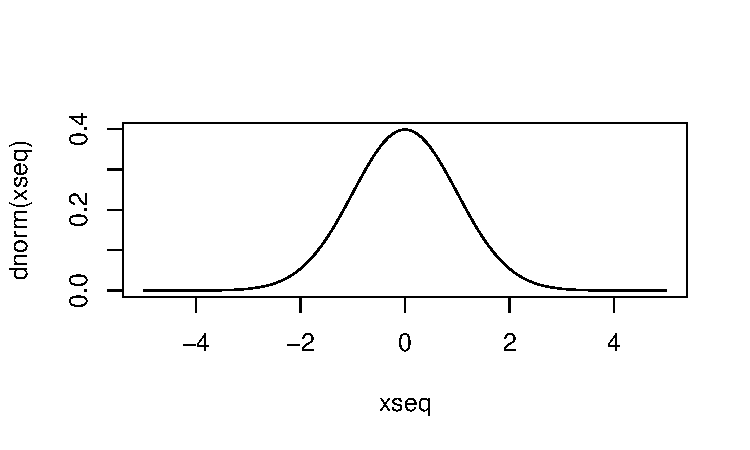
\includegraphics[width=0.7\linewidth]{Probability_Statistics_101_v2_files/figure-beamer/unnamed-chunk-15-1} \end{center}
\end{frame}

\begin{frame}
\frametitle{The Standard Normal Variable Z}

\begin{itemize}
\tightlist
\item
  \(\mu=0\) and \(\sigma=1\)
\item
  Example: find
  \[P(-1\leq Z \leq 1) = P(Z \leq 1) - P(Z < -1) = .842 - .159 \approx 68\% \]
\end{itemize}

\[P(-1.96\leq Z \leq 1.96) = .95 \]

\[P(-3 \leq Z \leq 3)  \approx 1 \]

Are those numbers familiar?
\end{frame}

\begin{frame}
\frametitle{A Normal Variable X}

\begin{itemize}
\tightlist
\item
  If \(X \sim N(\mu,\sigma^2)\), let \(Z = \frac{x - \mu}{\sigma}\),
  then \(Z \sim N(0,1)\)
\item
  So
  \[P(a \leq X \leq b) = P(\frac{a - \mu}{\sigma} \leq Z \leq \frac{b - \mu}{\sigma})\]
\item
  \[P(\mu - 1\sigma \leq X \leq \mu + 1\sigma) = P(-1 \leq Z \leq 1) = 68\%\]
  \[P(\mu - 2\sigma \leq X \leq \mu + 2\sigma) = P(-2 \leq Z \leq 2) = 95\%\]
  \[P(\mu - 3\sigma \leq X \leq \mu + 3\sigma) = P(-3 \leq Z \leq 3) = 100\%\]
\end{itemize}
\end{frame}

\begin{frame}
\frametitle{Distribution, mean and variance of $\bar{Y}_n$}

Example: If we play Red and Black games 100 times, we agree that the
average winning \(\bar{Y}_{100}\) follows a normal distribution with
mean being

\[
E(\bar{Y}_{100}) = \mu = -.0526
\] and a variance of \[
Var(\bar{Y}_{100}) = 0.997/100 \approx 0.01
\] \[
\sigma_{\bar{Y}_{100}} = \sqrt{0.01} = .1
\]

So \[
\bar{Y}_{100} \sim N(-.0526, 0.01)
\]
\end{frame}

\begin{frame}
\frametitle{Distribution, mean and variance of $\bar{X}_n$}

Example: If we play a single number game 100 times, we agree that the
average winning \(\bar{X}_{100}\) follows a normal distribution with
mean being

\[
E(\bar{X}_{100}) = \mu = -.0526
\] and a variance of \[
\sigma_{\bar{X}_{100}} = 5.76/\sqrt{100} = .576
\]

So \[
\bar{X}_{100} \sim N(-.0526, 0.576^2)
\]
\end{frame}

\begin{frame}
\frametitle{Comparison of two games}

\begin{itemize}
\tightlist
\item
  95\% of time

  \begin{itemize}
  \tightlist
  \item
    \(\bar{Y}_{100}\) will be within
    \(-.0526 \pm 2\times .1 = (-.25, .147)\)
  \item
    \(\bar{X}_{100}\) will be within
    \(-.0526 \pm 2\times .576 = (-1.2, 1.09)\)
  \end{itemize}
\item
  The chance for \(\bar{Y}_{100} > .147\) is same as
  \(\bar{X}_{100} > 1.09\), being 2.5\%
\end{itemize}

\begin{center}
Again, which game will you play?
\end{center}
\end{frame}

\begin{frame}
\frametitle{More detailed calculations:}

We can also find out:

\begin{enumerate}
[a)]
\tightlist
\item
  Prob (positive winning)=Prob(\(\bar{Y}_{100} > 0\) )
\item
  Prob (losing money)=Prob(\(\bar{Y}_{100} \leq 0\) )
\item
  Prob(\(-.2 \leq \bar{Y}_{100} \leq -.1\) )
\end{enumerate}
\end{frame}

\begin{frame}[fragile]
\frametitle{Red and Black games 100 times}

Recall \(\bar{Y}_{100} \sim N(-.0526, 0.01)\).

\begin{enumerate}
[a)]
\tightlist
\item
  Prob (positive winning)=Prob(\(\bar{Y}_{100} > 0\) )
\end{enumerate}

\[\begin{split}
P(\bar{Y}_{100} \geq 0) &=
P\left(Z \geq \frac{0-(-.0526)}{.1} \right) \\
&= P\left(Z \geq .526 \right) = .3
\end{split}\]

\begin{Shaded}
\begin{Highlighting}[]
\FunctionTok{pnorm}\NormalTok{(.}\DecValTok{526}\NormalTok{, }\AttributeTok{lower.tail =}\NormalTok{ F)}
\end{Highlighting}
\end{Shaded}

\begin{verbatim}
## [1] 0.2994441
\end{verbatim}

\begin{Shaded}
\begin{Highlighting}[]
\CommentTok{\# pnorm(0, mean = {-}.0526, sd = .1, lower.tail = F)}
\end{Highlighting}
\end{Shaded}
\end{frame}

\begin{frame}[fragile]
\frametitle{Red and Black games 100 times}

\begin{enumerate}
[(a)]
\setcounter{enumi}{1}
\tightlist
\item
  Prob (losing money)=Prob(\(\bar{Y}_{100} \leq 0\) ) = 1-
  Prob(\(\bar{Y}_{100} > 0\)) =1-.3=.7
\end{enumerate}

On average the chance to lose money is 70\%.

\begin{enumerate}
[a)]
\setcounter{enumi}{2}
\tightlist
\item
  Prob(\(-.2 \leq \bar{Y}_{100} \leq -.1\))
\end{enumerate}

\[\begin{split}
P(-.2 \leq \bar{Y}_{100} \leq -.1) &=
P\left(\frac{-.2-(-.0526)}{.1} \leq Z \leq \frac{-.1-(-.0526)}{.1} \right) \\
&= P\left(-1.474 \leq Z \leq -.474 \right) = .32 - .07 = .25
\end{split}\]

\begin{Shaded}
\begin{Highlighting}[]
\FunctionTok{pnorm}\NormalTok{(}\SpecialCharTok{{-}}\NormalTok{.}\DecValTok{474}\NormalTok{) }\SpecialCharTok{{-}} \FunctionTok{pnorm}\NormalTok{(}\SpecialCharTok{{-}}\FloatTok{1.474}\NormalTok{)}
\end{Highlighting}
\end{Shaded}

\begin{verbatim}
## [1] 0.2475092
\end{verbatim}

The chance of loosing between 10 and 20 cents on average is 25\%
\end{frame}

\begin{frame}
\frametitle{Single number game 100 times}

Recall \(\bar{X}_{100} \sim N(-.0526, 0.576^2)\).

Prob(losing money):

\[\begin{split}
P(\bar{X}_{100} < 0) &=
P\left(Z < \frac{0-(-.0526)}{.576} \right) \\
&= P\left(Z \geq .0913 \right) = .536
\end{split}\]

On average the chance to lose money is 53.6\%!
\end{frame}

\hypertarget{stat-101-confidence-intervals-hypothesis-tests}{%
\section{Stat 101: Confidence Intervals, Hypothesis
Tests}\label{stat-101-confidence-intervals-hypothesis-tests}}

\begin{frame}
\frametitle{Is the Casino being honest?}

Case: Linda played roulette 100 times

\begin{itemize}
\item
  \$1 bet each time on Red/Black
\item
  She lost \$28
\item
  She knew the roulette table is a biased one. HOW????
\end{itemize}

\footnotesize
\end{frame}

\hypertarget{confidence-interval}{%
\subsection{Confidence Interval}\label{confidence-interval}}

\begin{frame}
\frametitle{95\% Confidence interval}

\(\bar{X}\) has a normal distribution with \(\mu\) and
\(sd =\frac{\sigma}{\sqrt{100}} = \frac{.998}{10} \approx .1\)

Which means 95\% of time \[|\bar{X} - \mu| < 1.96 \times .1\]

This is same to say 95\% time the mean \(\mu\) should be in
\[\bar{X} \pm 1.96 \times \frac{\sigma}{\sqrt{100}} = (\bar{X} - .2, \bar{X} + .2)\]

Apply to our data, we have a 95\% confidence interval (z):
\[-.28 \pm 2\times .1 = (-.48, -.08)\]

Conclusion: The roulette is not fair. 95\% CI does not contain -.0526.
\end{frame}

\begin{frame}
\frametitle{$t$-Confidence interval}

\begin{itemize}
\item
  \(\sigma\) is not known either, we estimate \(\sigma\) by \(s=.965\)
\item
  We will have a \(t\)-interval:
  \[\bar{X} \pm t_{df} \times \frac{s}{\sqrt{100}} = -.28 \pm 1.98 \times \frac{.965}{\sqrt{100}} = (-.471, -.089)\]
\item
  We have the same conclusion that the wheel is not a fair one since the
  true mean -.0526 in not in the interval.
\item
  \(t\) intervals are wider than \(z\) intervals
\end{itemize}
\end{frame}

\begin{frame}
\end{frame}

\hypertarget{hypothesis-tests}{%
\subsection{Hypothesis tests}\label{hypothesis-tests}}

\begin{frame}{Hypothesis tests}
\frametitle{Hypotheses testing}

\begin{itemize}
\item
  We may ask is it possible that\(\mu=-.0526\)?
\item
  \(H_0: \mu = -.0526 \quad \mbox{vs.} \quad H_1: \mu \neq -.0526\)
\item
  Testing statistics \[
  Z = \frac{\bar{X} - (-.0526)}{s/\sqrt{n}} = \frac{-.28 + .0526}{.998/{/sqrt{100}}} = -2.28
  \]
\item
  \(p\mbox{-value}=P(|Z|> 2.28) =.022\) if \(\mu = -.0526\)
\item
  Conclusion: Since \(p\)-value is so small, we reject \(H_0\).
\end{itemize}
\end{frame}

\hypertarget{appendix}{%
\section{Appendix}\label{appendix}}

\begin{frame}
\frametitle{Bernoulli Distribution}

The success of each bet \(X\) of the single number game or the Red-Black
game follows a Bernoulli distribution. Denote success as 1.

\begin{itemize}
\item
  Single number game
  \[X = \begin{cases} 1 & \text{with probability (w.p.) 1/38} \\
                    0 & \text{w.p. 37/38} \end{cases}\]
\item
  Red-Black game \[X = \begin{cases} 1 & \text{w.p. 18/38,} \\
                    0 & \text{w.p. 20/38} \end{cases}\]
\end{itemize}
\end{frame}

\begin{frame}[fragile]
\frametitle{Bernoulli Distribution}

Simulate 100 trials. Use \texttt{rbinom()} to generate random samples.

\small

\begin{verbatim}
##   [1] 0 1 1 1 1 0 0 1 1 0 1 1 0 1 1 1 0 0 0 1 1 1 1 1 1 0 0 0 0 0 0 0 0 1 0 1 1
##  [38] 0 0 0 1 0 1 1 1 1 0 1 1 0 0 0 1 1 1 0 0 1 1 1 0 1 0 1 0 0 0 0 1 0 1 0 1 1
##  [75] 0 1 1 0 1 0 0 1 1 1 1 0 1 1 1 1 0 0 0 0 1 1 0 1 1 1
\end{verbatim}
\end{frame}

\begin{frame}
\frametitle{Binomial Distribution}

If we bet 100 times, or say we draw 100 samples from the Bernoulli
distribution, the total number of success among these 100 times \(Y\)
follow binomial distribution. \[Y \sim Binomial(n, p) \] where \(n\) is
the total number of trials and \(p\) is the probability of success of
each trial.

\begin{itemize}
\item
  Single number game \[X = Binomial(100, 1/38)\]
\item
  Red-Black game \[X = Binomial(100, 18/38)\]
\end{itemize}
\end{frame}

\begin{frame}[fragile]
\frametitle{Binomial Distribution}

The probability of success \(k\) times among 100 trials is
\[Prob(Y=k) = 
\left(\begin{array}{c}
100\\
k
\end{array}\right) 
p^k (1-p)^{n-k}\]

\begin{verbatim}
## [1] 0.7349765
\end{verbatim}
\end{frame}

\begin{frame}[fragile]
\frametitle{Binomial Distribution}

Simulate total number of success among 100 trials. Use \texttt{rbinom()}
to generate random samples.

\small

\begin{verbatim}
## [1] 50
\end{verbatim}
\end{frame}

\begin{frame}
\frametitle{Covariances: $Cov(X_R, X_B)$}

\begin{itemize}
\item
  \(X_R\) = Winning over one dollar bet on Red
\item
  \(X_B\) = Winning over one dollar bet on Black
\item
  \(X_R\) and \(X_B\) are related: if \(X_R=1\), then \(X_B=-1\)
\item
  We use covariance to measure the relationship
  \[COV(X_R, X_B)=E(X_R-E(X_R)( X_B-E(X_B))\] \[COV(X_R, X_B)=-.8975\]
\item
  Or Correlation
  \[\rho = \frac{COV(X_R, X_B)}{SD(X_R) SD(X_B)} = \frac{-.8975}{.998 \times 998} = -.9011\]
\end{itemize}
\end{frame}

\begin{frame}
\frametitle{Correlation}

\[\rho = \frac{COV(X_R, X_B)}{SD(X_R) SD(X_B)} = \frac{-.8975}{.998 \times 998} = -.9011\]

\begin{itemize}
\tightlist
\item
  Correlation captures linear relationship between XR and XB
\item
  \(-1 < \rho < 1\)
\item
  The larger \(|\rho|\) is, the stronger of the relationship
\item
  The sign of \(\rho\) reflects the direction of associations
\end{itemize}
\end{frame}

\begin{frame}
\frametitle{$E(X_R+X_B)$ and $VAR(X_R+X_B)$}

\begin{itemize}
\tightlist
\item
  \(E(X_R+X_B)=E(X_R) + E(X_B)\)
\item
  \(VAR(X_R+X_B)= VAR(X_R)+ VAR(X_B)+2COV(X_R, X_B)\)
\item
  \(VAR(aX_R+bX_B)=a^2 VAR(X_R)+b^2 VAR(X_B) +2ab COV(X_R, X_B)\)
\item
  If X and Y are independent \(COV(X, Y)=0\)
  \(VAR(aX+bY)= a^2 VAR(X)+b^2 VAR(Y)\)
\item
  That is why \(Var(\bar{X}_n) = \frac{\sigma^2}{n}\)
\end{itemize}
\end{frame}

\end{document}
